\subsection{Variational Autoencoder}
\label{back:vae}

The \acrfull{vae} \cite{kingma2022autoencodingvariationalbayes} is a type of autoencoder that aims to solve the lack of generative capabilities within regular autoencoders. \acrshort{vae}s are generative models that sample the latent space through a probabilistic distribution. This makes them suitable for image generation tasks \cite{vahdat2020nvae}, something regular autoencoders are unable to do due to their deterministic latent representation.

\begin{figure}[!h]
    \centering
    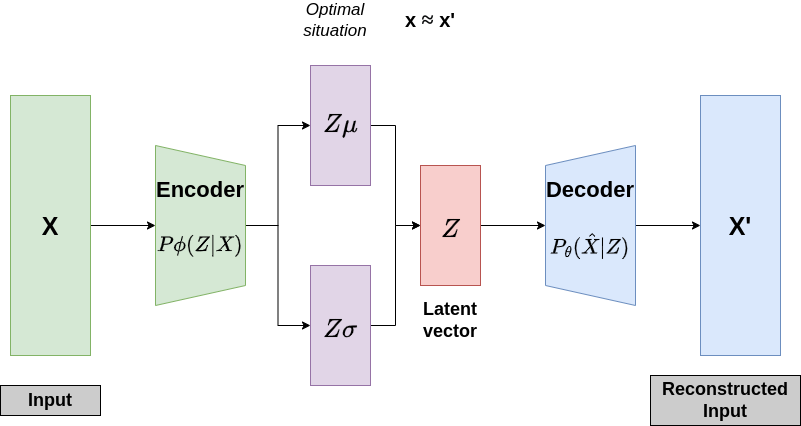
\includegraphics[scale=0.4]{figures/vae.png}
    \caption{Variational Autoencoder Architecture Diagram}
    \label{fig:vaediagram}
\end{figure}


\subsubsection{Reparametrization Trick}
\label{back:reparam}

\acrshort{vae}s can be trained efficiently using backpropagation due to a technique known as the \textit{reparameterization trick} \cite{kingma2022autoencodingvariationalbayes}. This is necessary because \acrshort{vae}s involve sampling from a stochastic latent variable $z$, which would normally hinder gradient-based optimization.

The idea is to express the sampling of $z$ from the approximate posterior $q_\phi(z|x) = \mathcal{N}(\mu, \sigma^2)$ as a deterministic function of the encoder outputs ($\mu$ and $\sigma$) and an additional noise variable $\epsilon$. Specifically:
\begin{equation}
    z = \mu + \sigma \odot \epsilon, \quad \epsilon \sim \mathcal{N}(0, I)
\end{equation}

Here, $\odot$ denotes element-wise multiplication. This formulation allows gradients to flow through the sampling process, enabling end-to-end training of the model.

The reparameterization trick transforms the optimization problem from one involving expectations over $q_\phi(z|x)$ to one involving expectations over $p(\epsilon)$, which is fixed and independent of the model parameters ($\phi$ and $\theta$):

\begin{equation}
    \mathbb{E}_{z \sim q_\phi(z|x)}[f(z)] = \mathbb{E}_{\epsilon \sim \mathcal{N}(0,I)}[f(\mu + \sigma \odot \epsilon)]
\end{equation}

This formulation makes training of \acrshort{vae} models feasable, even for gradient based optimizers, such as \acrshort{adam} or \acrshort{sgd}.




\subsubsection{Evidence Lower Bound}
\label{back:elbo}
In the context of \acrshort{vae}s, \acrshort{elbo} is commonly used as a loss function. \cite{lygerakis2024edvaeentropydecompositionelbo}. It consists of two parts, the reconstruction likelihood $\mathcal{L}_{\text{rec}}$ and the prior constraint $\mathcal{L}_{\text{reg}}$:
\begin{align}
\mathcal{L}_{\text{ELBO}}(\theta, \phi; x) &= \mathcal{L}_{\text{rec}}(\theta, \phi; x) + \mathcal{L}_{\text{reg}}(\phi; x)  
\end{align}
where:
\begin{align}
\mathcal{L}_{\text{rec}}(\theta, \phi; x) &= \mathbb{E}_{q_\phi(z|x)}[\log p_\theta(x|z)] \\
\mathcal{L}_{\text{reg}}(\phi; x) &= -D_{\text{KL}}(q_\phi(z|x) \| p(z))
\end{align}
$\mathcal{L}_{\text{reg}}$ is the negative \acrfull{kld} \cite{10.1214/aoms/1177729694}, which can be further formulated as:
\begin{equation}
    D_{\text{KL}}(q_\phi(z|x) \| p(z)) = \mathbb{E}_{q_\phi(z|x)}\left[\log \frac{q_\phi(z|x)}{p(z)}\right]
\end{equation}
$D_{\text{KL}}$ is always non-negative $(\geq 0)$ and is a statistical method used to quantify the proximity between two probability distributions \cite{shlens2014notes}. 
The reconstruction likelihood $\mathcal{L}_{\text{rec}}$ can be computed in different ways depending on the nature of the input data. For binary data, it is typically computed as a binary cross-entropy loss:
\begin{equation}
\mathcal{L_\text{rec}}(\theta, \phi; x) = - \mathbb{E}_{q_\phi(z|x)}[\mathcal{L}_{\text{BCE}}(x, z)]
\end{equation}
where $\mathcal{L}_{\text{BCE}}(x, z)$ is defined as:
\begin{equation}
\mathcal{L}_{\text{BCE}}(x, z) = \frac{1}{N} \sum_{i=1}^{N} \left( x_i \log p_\theta(x_i|z) + (1 - x_i) \log(1 - p_\theta(x_i|z)) \right)
\end{equation}
For continuous data, more novel adaptations \cite{lygerakis2024edvaeentropydecompositionelbo} often use the \acrshort{mse} loss as shown in equation \ref{eq:mse}, thus giving:
\begin{equation}
    \mathcal{L}_{\text{rec}}(\theta, \phi; x) = \mathbb{E}_{q_\phi(z|x)}[\|x - \hat{x}\|^2]
\end{equation}
where $\hat{x} = p_\theta(x|z)$ is the reconstructed input.
The two losses combined aims at providing a total loss that balances reconstruction quality and the prior regularization \cite{lin2019balancingreconstructionqualityregularisation}.

\subsubsection{Minimizing the ELBO Loss}
The objective in training a \acrshort{vae} is to minimize the negative \acrshort{elbo}, which is equivalent to maximizing the \acrshort{elbo} itself. This optimization problem can be formulated as:

\begin{equation}
    \theta^*, \phi^* = \argmin_{\theta, \phi} \mathbb{E}_{x \sim p_{\text{data}}(x)}[-\mathcal{L}_{\text{ELBO}}(\theta, \phi; x)]
\end{equation}

where $\theta^*$ and $\phi^*$ are the optimal parameters for the decoder and encoder, respectively. By minimizing the negative \acrshort{elbo}, we simultaneously optimize for better reconstruction of the input data (through $\mathcal{L}_{\text{rec}}$) and a latent space distribution that closely matches the prior (through $\mathcal{L}_{\text{reg}}$). This process encourages the \acrshort{vae} to learn a meaningful and structured latent representation of the input data while maintaining the ability to generate new samples \cite{kingma2022autoencodingvariationalbayes}.